\documentclass[12pt]{article}
\usepackage[paperwidth=55cm,paperheight=78cm,margin=1cm]{geometry}
\usepackage{tikz}
\usepackage{amsmath,amssymb}
\usepackage[T1]{fontenc}
\usepackage{helvet}
\renewcommand{\familydefault}{\sfdefault}

\usetikzlibrary{shapes.geometric,arrows.meta,positioning,fit,backgrounds,calc}

\definecolor{cBlue}{HTML}{2980b9}
\definecolor{cBlueBg}{HTML}{d6eaf8}
\definecolor{cGreen}{HTML}{1a9876}
\definecolor{cGreenBg}{HTML}{d0ece7}
\definecolor{cOrange}{HTML}{d35400}
\definecolor{cOrangeBg}{HTML}{fdebd0}
\definecolor{cRed}{HTML}{c0392b}
\definecolor{cRedBg}{HTML}{fadbd8}
\definecolor{cPurple}{HTML}{6c3483}
\definecolor{cPurpleBg}{HTML}{e8daef}
\definecolor{cGold}{HTML}{b7950b}
\definecolor{cGoldBg}{HTML}{fef9e7}
\definecolor{cTeal}{HTML}{148f77}
\definecolor{cArrow}{HTML}{2c3e50}
\definecolor{cLoopBg}{HTML}{f5eef8}

\pagestyle{empty}

\begin{document}
\begin{center}
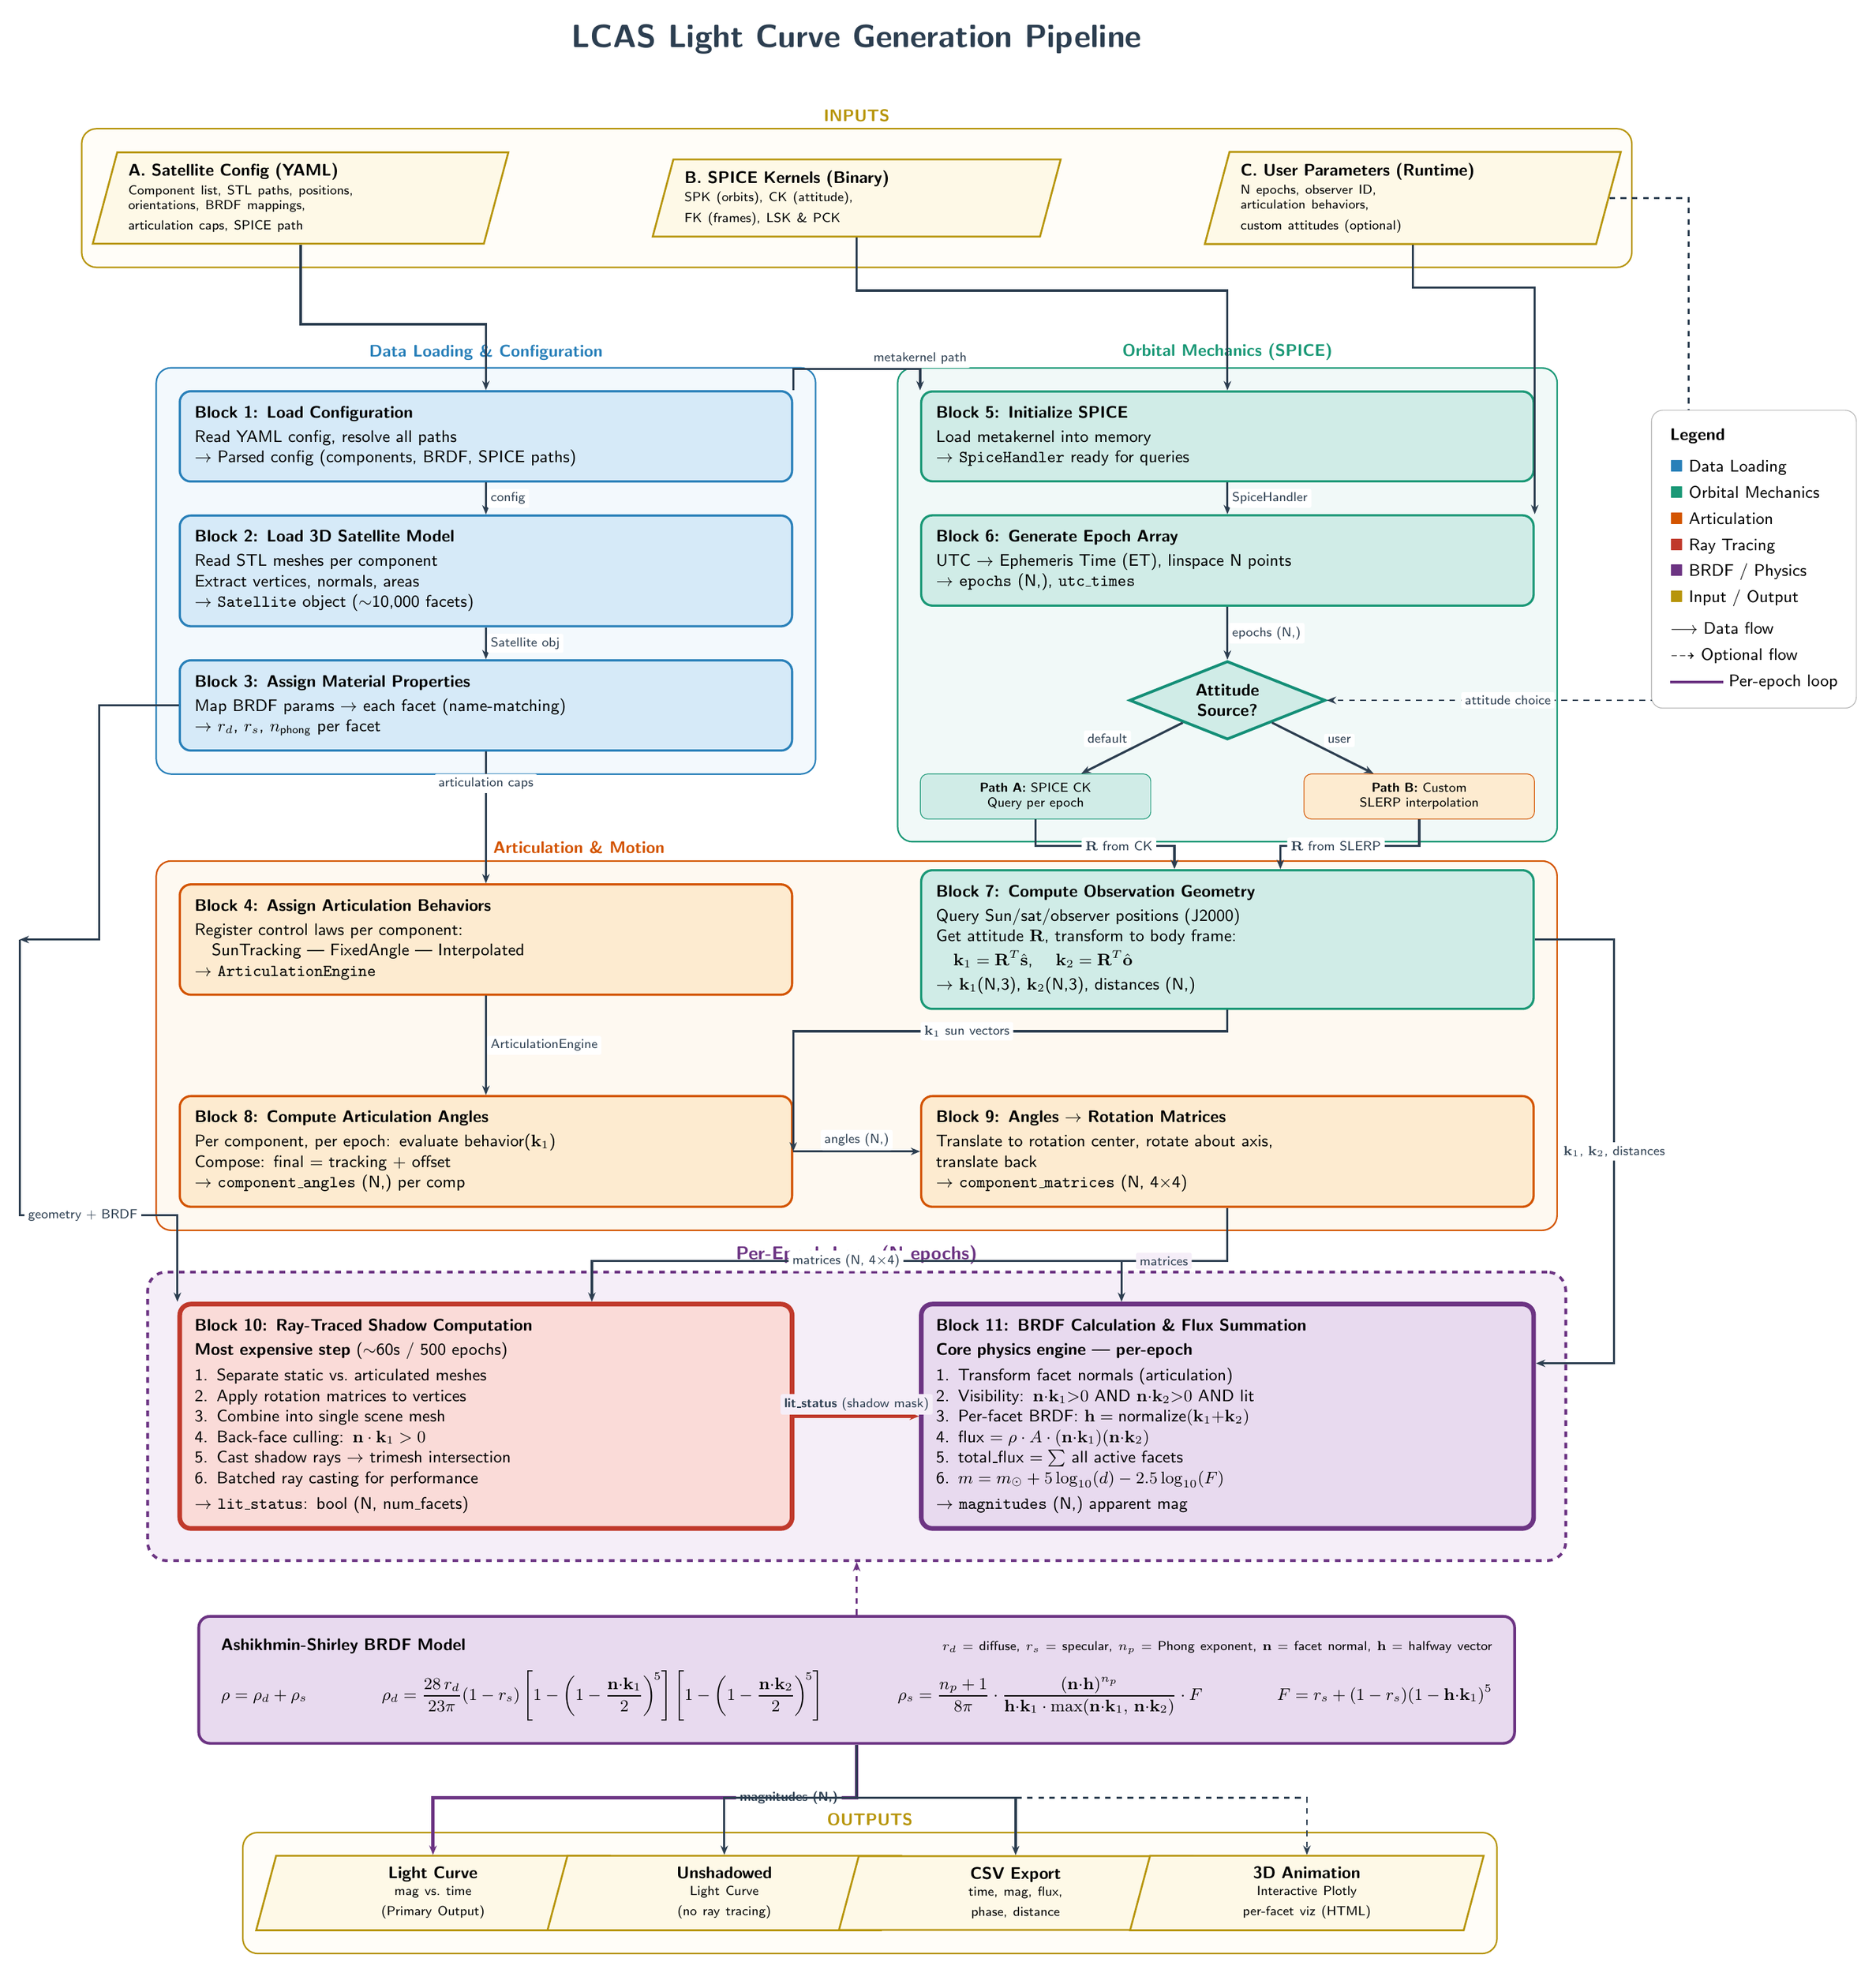
\begin{tikzpicture}[
    arr/.style={-{Stealth[length=5pt,width=4pt]}, line width=1.2pt, color=cArrow},
    darr/.style={-{Stealth[length=5pt,width=4pt]}, line width=1pt, color=cArrow, dashed},
    lbl/.style={font=\scriptsize\sffamily, text=cArrow, fill=white, inner sep=2pt, rounded corners=1pt},
    lblc/.style={font=\scriptsize\sffamily, text=cArrow, fill=cLoopBg, inner sep=2pt, rounded corners=1pt},
    inputbox/.style={
        trapezium, trapezium left angle=75, trapezium right angle=105,
        draw=cGold, line width=1pt, fill=cGoldBg,
        text width=6.5cm, minimum height=1cm,
        inner sep=6pt, font=\small, align=left
    },
    outputbox/.style={
        trapezium, trapezium left angle=75, trapezium right angle=105,
        draw=cGold, line width=1pt, fill=cGoldBg,
        text width=5.5cm, minimum height=1cm,
        inner sep=6pt, font=\small, align=center
    },
    decision/.style={
        diamond, draw=cTeal, line width=1.5pt,
        fill=cGreenBg, inner sep=4pt,
        font=\small\bfseries, aspect=2.5, align=center
    },
    hblock/.style={
        rectangle, rounded corners=6pt,
        draw=#1, line width=1.2pt, fill=#1Bg,
        text width=11cm, inner sep=8pt, font=\small, align=left
    },
    bblock/.style={
        rectangle, rounded corners=6pt,
        draw=#1, line width=2.5pt, fill=#1Bg,
        text width=11cm, inner sep=8pt, font=\small, align=left
    }
]

% ═══════════ TITLE ═══════════
\node[font=\LARGE\bfseries, text=cArrow] (title) at (0, 0) 
    {LCAS Light Curve Generation Pipeline};

% ═══════════ INPUTS ═══════════
\node[inputbox] (inA) at (-10.5, -3) {%
    \textbf{A. Satellite Config (YAML)}\\[2pt]
    {\scriptsize Component list, STL paths, positions,\\
    orientations, BRDF mappings,\\
    articulation caps, SPICE path}};
\node[inputbox] (inB) at (0, -3) {%
    \textbf{B. SPICE Kernels (Binary)}\\[2pt]
    {\scriptsize SPK (orbits), CK (attitude),\\
    FK (frames), LSK \& PCK}};
\node[inputbox] (inC) at (10.5, -3) {%
    \textbf{C. User Parameters (Runtime)}\\[2pt]
    {\scriptsize N epochs, observer ID,\\
    articulation behaviors,\\
    custom attitudes (optional)}};

\begin{scope}[on background layer]
    \node[fit=(inA)(inB)(inC), fill=cGoldBg!30, draw=cGold, 
          rounded corners=8pt, inner sep=12pt, line width=0.8pt,
          label={[font=\small\bfseries,text=cGold]above:INPUTS}] {};
\end{scope}

% ═══════════ ROW 2: LEFT = Loading, RIGHT = SPICE ═══════════
% Left column (x = -7)
\node[hblock=cBlue] (B1) at (-7, -7.5) {%
    \textbf{Block 1: Load Configuration}\\[2pt]
    Read YAML config, resolve all paths\\
    $\rightarrow$ Parsed config (components, BRDF, SPICE paths)};

\node[hblock=cBlue, below=0.6cm of B1] (B2) {%
    \textbf{Block 2: Load 3D Satellite Model}\\[2pt]
    Read STL meshes per component\\
    Extract vertices, normals, areas\\
    $\rightarrow$ \texttt{Satellite} object ($\sim$10{,}000 facets)};

\node[hblock=cBlue, below=0.6cm of B2] (B3) {%
    \textbf{Block 3: Assign Material Properties}\\[2pt]
    Map BRDF params $\rightarrow$ each facet (name-matching)\\
    $\rightarrow$ $r_d$, $r_s$, $n_{\text{phong}}$ per facet};

\begin{scope}[on background layer]
    \node[fit=(B1)(B2)(B3), fill=cBlueBg!30, draw=cBlue, 
          rounded corners=8pt, inner sep=12pt, line width=0.8pt,
          label={[font=\small\bfseries,text=cBlue]above:Data Loading \& Configuration}] {};
\end{scope}

% Right column (x = 7)
\node[hblock=cGreen] (B5) at (7, -7.5) {%
    \textbf{Block 5: Initialize SPICE}\\[2pt]
    Load metakernel into memory\\
    $\rightarrow$ \texttt{SpiceHandler} ready for queries};

\node[hblock=cGreen, below=0.6cm of B5] (B6) {%
    \textbf{Block 6: Generate Epoch Array}\\[2pt]
    UTC $\rightarrow$ Ephemeris Time (ET), linspace N points\\
    $\rightarrow$ \texttt{epochs} (N,), \texttt{utc\_times}};

\node[decision, below=1cm of B6] (att) {Attitude\\Source?};

\node[rectangle, rounded corners=4pt, draw=cGreen, fill=cGreenBg,
      font=\scriptsize, text width=4cm, align=center, inner sep=5pt,
      below left=1cm and 0.5cm of att] (pathA) {\textbf{Path A:} SPICE CK\\Query per epoch};
\node[rectangle, rounded corners=4pt, draw=cOrange, fill=cOrangeBg,
      font=\scriptsize, text width=4cm, align=center, inner sep=5pt,
      below right=1cm and 0.5cm of att] (pathB) {\textbf{Path B:} Custom\\SLERP interpolation};

\begin{scope}[on background layer]
    \node[fit=(B5)(B6)(att)(pathA)(pathB), fill=cGreenBg!30, draw=cGreen,
          rounded corners=8pt, inner sep=12pt, line width=0.8pt,
          label={[font=\small\bfseries,text=cGreen]above:Orbital Mechanics (SPICE)}] {};
\end{scope}

% Row 2 internal arrows
\draw[arr] (B1) -- node[lbl,right] {config} (B2);
\draw[arr] (B2) -- node[lbl,right] {Satellite obj} (B3);
\draw[arr] (B5) -- node[lbl,right] {SpiceHandler} (B6);
\draw[arr] (B6) -- node[lbl,right] {epochs (N,)} (att);
\draw[arr] (att) -- node[lbl,above left] {default} (pathA);
\draw[arr] (att) -- node[lbl,above right] {user} (pathB);

% Input arrows — straight drops into their columns
\draw[arr] (inA.south) -- ++(0,-1.5) -| (B1.north);
\draw[arr] (inB.south) -- ++(0,-1) -| (B5.north);
\draw[arr] (inC.south) -- ++(0,-0.8) -| (B6.north east);

% Cross-column: B1 metakernel → B5 (route above the boxes)
\draw[arr] (B1.north east) -- ++(0,0.4) -| node[lbl, pos=0.5, above] {metakernel path} (B5.north west);

% ═══════════ ROW 3: Block 4 + Block 7 ═══════════
\node[hblock=cOrange] (B4) at (-7, -17) {%
    \textbf{Block 4: Assign Articulation Behaviors}\\[2pt]
    Register control laws per component:\\
    \quad SunTracking | FixedAngle | Interpolated\\
    $\rightarrow$ \texttt{ArticulationEngine}};

\node[hblock=cGreen] (B7) at (7, -17) {%
    \textbf{Block 7: Compute Observation Geometry}\\[2pt]
    Query Sun/sat/observer positions (J2000)\\
    Get attitude $\mathbf{R}$, transform to body frame:\\[2pt]
    \quad $\mathbf{k}_1 = \mathbf{R}^T \hat{\mathbf{s}}$, \quad
    $\mathbf{k}_2 = \mathbf{R}^T \hat{\mathbf{o}}$\\[2pt]
    $\rightarrow$ $\mathbf{k}_1$(N,3), $\mathbf{k}_2$(N,3), distances (N,)};

% B1 → B4 arrow (down left side)
\draw[arr] (B3.south) -- ++(0,-0.6) -| node[lbl, pos=0.25] {articulation caps} (B4.north);

% Attitude paths → B7
\draw[arr] (pathA.south) -- ++(0,-0.5) -| node[lbl, pos=0.3] {$\mathbf{R}$ from CK} ([xshift=-1cm]B7.north);
\draw[arr] (pathB.south) -- ++(0,-0.5) -| node[lbl, pos=0.3] {$\mathbf{R}$ from SLERP} ([xshift=1cm]B7.north);

% Attitude choice dashed arrow (from far right, loops around)
\draw[darr] (inC.east) -- ++(1.5,0) |- node[lbl, pos=0.75] {attitude choice} (att.east);

% ═══════════ ROW 4: Blocks 8, 9 ═══════════
\node[hblock=cOrange] (B8) at (-7, -21) {%
    \textbf{Block 8: Compute Articulation Angles}\\[2pt]
    Per component, per epoch: evaluate behavior($\mathbf{k}_1$)\\
    Compose: final = tracking + offset\\
    $\rightarrow$ \texttt{component\_angles} (N,) per comp};

\node[hblock=cOrange] (B9) at (7, -21) {%
    \textbf{Block 9: Angles $\rightarrow$ Rotation Matrices}\\[2pt]
    Translate to rotation center, rotate about axis,\\
    translate back\\
    $\rightarrow$ \texttt{component\_matrices} (N, 4$\times$4)};

\begin{scope}[on background layer]
    \node[fit=(B4)(B8)(B9), fill=cOrangeBg!30, draw=cOrange,
          rounded corners=8pt, inner sep=12pt, line width=0.8pt,
          label={[font=\small\bfseries,text=cOrange]above left:Articulation \& Motion}] {};
\end{scope}

% Row 3→4 arrows
\draw[arr] (B4) -- node[lbl,right] {ArticulationEngine} (B8);
\draw[arr] (B7.south) -- ++(0,-0.4) -| node[lbl, pos=0.3] {$\mathbf{k}_1$ sun vectors} (B8.east);
\draw[arr] (B8) -- node[lbl,above] {angles (N,)} (B9);

% ═══════════ ROW 5: Core (Blocks 10, 11) ═══════════
\node[bblock=cRed] (B10) at (-7, -26) {%
    \textbf{Block 10: Ray-Traced Shadow Computation}\\[2pt]
    \textbf{Most expensive step} ($\sim$60s / 500 epochs)\\[3pt]
    1. Separate static vs.\ articulated meshes\\
    2. Apply rotation matrices to vertices\\
    3. Combine into single scene mesh\\
    4. Back-face culling: $\mathbf{n} \cdot \mathbf{k}_1 > 0$\\
    5. Cast shadow rays $\rightarrow$ trimesh intersection\\
    6. Batched ray casting for performance\\[3pt]
    $\rightarrow$ \texttt{lit\_status}: bool (N, num\_facets)};

\node[bblock=cPurple] (B11) at (7, -26) {%
    \textbf{Block 11: BRDF Calculation \& Flux Summation}\\[2pt]
    \textbf{Core physics engine --- per-epoch}\\[3pt]
    1. Transform facet normals (articulation)\\
    2. Visibility: $\mathbf{n}{\cdot}\mathbf{k}_1{>}0$ AND $\mathbf{n}{\cdot}\mathbf{k}_2{>}0$ AND lit\\
    3. Per-facet BRDF: $\mathbf{h} = \text{normalize}(\mathbf{k}_1{+}\mathbf{k}_2)$\\
    4. flux $= \rho \cdot A \cdot (\mathbf{n}{\cdot}\mathbf{k}_1)(\mathbf{n}{\cdot}\mathbf{k}_2)$\\
    5. total\_flux $= \sum$ all active facets\\
    6. $m = m_\odot + 5\log_{10}(d) - 2.5\log_{10}(F)$\\[3pt]
    $\rightarrow$ \texttt{magnitudes} (N,) apparent mag};

\begin{scope}[on background layer]
    \node[fit=(B10)(B11), fill=cLoopBg, draw=cPurple,
          rounded corners=10pt, inner sep=16pt, line width=1.5pt, dashed,
          label={[font=\normalsize\bfseries,text=cPurple]above:Per-Epoch Loop (N epochs)}] (loopbox) {};
\end{scope}

% Core arrows
\draw[arr, color=cRed, line width=1.8pt] (B10) -- node[lblc,above] {\textbf{lit\_status} (shadow mask)} (B11);

% B3 → B10 (down the left side, outside articulation box)
\draw[arr] ([xshift=-3cm]B4.west) -- ++(0,-5.2) -| node[lbl, pos=0.2] {geometry + BRDF} (B10.north west);
\draw[arr] (B3.west) -- ++(-1.5,0) |- ([xshift=-3cm]B4.west);

% B9 → B10 and B9 → B11
\draw[arr] (B9.south) -- ++(0,-1) -| node[lbl, pos=0.3] {matrices (N, 4$\times$4)} ([xshift=2cm]B10.north);
\draw[arr] (B9.south) -- ++(0,-1) -| node[lblc, pos=0.3] {matrices} ([xshift=-2cm]B11.north);

% B7 → B11 (down the right side, outside boxes)
\draw[arr] (B7.east) -- ++(1.5,0) |- node[lbl, pos=0.25] {$\mathbf{k}_1$, $\mathbf{k}_2$, distances} ([yshift=1cm]B11.east);

% ═══════════ BRDF Formula ═══════════
\node[rectangle, rounded corners=6pt, draw=cPurple, line width=1.5pt,
      fill=cPurpleBg, text width=24cm, inner sep=12pt, font=\small,
      below=1cm of loopbox] (brdf) {%
    \textbf{Ashikhmin-Shirley BRDF Model} \hfill 
    {\scriptsize $r_d$ = diffuse, $r_s$ = specular, $n_p$ = Phong exponent, 
    $\mathbf{n}$ = facet normal, $\mathbf{h}$ = halfway vector}\\[8pt]
    $\displaystyle \rho = \rho_d + \rho_s$ \qquad\qquad
    $\displaystyle \rho_d = \frac{28\, r_d}{23\pi}(1 - r_s)
        \left[1 - \left(1 - \frac{\mathbf{n}{\cdot}\mathbf{k}_1}{2}\right)^{\!5}\right]
        \left[1 - \left(1 - \frac{\mathbf{n}{\cdot}\mathbf{k}_2}{2}\right)^{\!5}\right]$
    \qquad\qquad
    $\displaystyle \rho_s = \frac{n_p + 1}{8\pi}
        \cdot \frac{(\mathbf{n}{\cdot}\mathbf{h})^{n_p}}
        {\mathbf{h}{\cdot}\mathbf{k}_1 \cdot \max(\mathbf{n}{\cdot}\mathbf{k}_1,\, \mathbf{n}{\cdot}\mathbf{k}_2)}
        \cdot F$
    \qquad\qquad
    $\displaystyle F = r_s + (1 - r_s)(1 - \mathbf{h}{\cdot}\mathbf{k}_1)^5$};
\draw[darr, color=cPurple] (brdf.north) -- (loopbox.south);

% ═══════════ OUTPUTS ═══════════
\node[outputbox] (outLC) at (-8, -35) {%
    \textbf{Light Curve}\\[1pt]
    {\scriptsize mag vs.\ time\\(Primary Output)}};
\node[outputbox] (outUS) at (-2.5, -35) {%
    \textbf{Unshadowed}\\[1pt]
    {\scriptsize Light Curve\\(no ray tracing)}};
\node[outputbox] (outCSV) at (3, -35) {%
    \textbf{CSV Export}\\[1pt]
    {\scriptsize time, mag, flux,\\phase, distance}};
\node[outputbox] (outAnim) at (8.5, -35) {%
    \textbf{3D Animation}\\[1pt]
    {\scriptsize Interactive Plotly\\per-facet viz (HTML)}};

\begin{scope}[on background layer]
    \node[fit=(outLC)(outUS)(outCSV)(outAnim), fill=cGoldBg!30, draw=cGold,
          rounded corners=8pt, inner sep=12pt, line width=0.8pt,
          label={[font=\small\bfseries,text=cGold]above:OUTPUTS}] {};
\end{scope}

% Output arrows — from brdf box down
\draw[arr, line width=1.8pt, color=cPurple] (brdf.south) -- ++(0,-1) -| node[lbl, pos=0.08] {\textbf{magnitudes (N,)}} (outLC.north);
\draw[arr] (brdf.south) -- ++(0,-1) -| (outUS.north);
\draw[arr] (brdf.south) -- ++(0,-1) -| (outCSV.north);
\draw[darr] (brdf.south) -- ++(0,-1) -| (outAnim.north);

% ═══════════ LEGEND (far right, clear of everything) ═══════════
\node[rectangle, rounded corners=6pt, draw=gray!60, fill=white, 
      inner sep=10pt, font=\small, align=left,
      anchor=north west] at (15, -7) {%
    \textbf{Legend}\\[6pt]
    \textcolor{cBlue}{$\blacksquare$} Data Loading\\[3pt]
    \textcolor{cGreen}{$\blacksquare$} Orbital Mechanics\\[3pt]
    \textcolor{cOrange}{$\blacksquare$} Articulation\\[3pt]
    \textcolor{cRed}{$\blacksquare$} Ray Tracing\\[3pt]
    \textcolor{cPurple}{$\blacksquare$} BRDF / Physics\\[3pt]
    \textcolor{cGold}{$\blacksquare$} Input / Output\\[6pt]
    $\longrightarrow$ Data flow\\[3pt]
    $\dashrightarrow$ Optional flow\\[3pt]
    {\color{cPurple}\rule[0.4ex]{1cm}{1.5pt}} Per-epoch loop};

\end{tikzpicture}
\end{center}
\end{document}
